\documentclass[10pt]{article}

% amsmath package, useful for mathematical formulas
\usepackage{amsmath}
% amssymb package, useful for mathematical symbols
\usepackage{amssymb}

% graphicx package, useful for including eps and pdf graphics
% include graphics with the command \includegraphics
\usepackage{graphicx}
\usepackage{epstopdf}
\graphicspath{ {./figures/} }

% cite package, to clean up citations in the main text. Do not remove.
\usepackage{cite}
\usepackage{color}
\usepackage{soul}
\usepackage{longtable}
\usepackage{pdfpages}
\usepackage{color}

% Text layout
\topmargin 0.0cm
\oddsidemargin 0.5cm
\evensidemargin 0.5cm
\textwidth 16cm 
\textheight 21cm

% Bold the 'Figure #' in the caption and separate it with a period
% Captions will be left justified
\usepackage[labelfont=bf,labelsep=period,justification=raggedright]{caption}


\bibliographystyle{plain}

% Remove brackets from numbering in List of References
\makeatletter
\renewcommand{\@biblabel}[1]{\quad#1.}
\makeatother


% Leave date blank
\date{}

\pagestyle{myheadings}
%% ** EDIT HERE **

\newcommand{\beginsupplement}{%
        \setcounter{table}{0}
        \renewcommand{\thetable}{S\arabic{table}}%
        \setcounter{figure}{0}
        \renewcommand{\thefigure}{S\arabic{figure}}%
     }


%% END MACROS SECTION

\begin{document}

\begin{flushleft}
{\Large
\textbf{The Metabolic Landscape of Tumors}
}
% Insert Author names, affiliations and corresponding author email.
\\
E Reznik, A Luna, BA Aksoy, C Sander, others less worthy
\\
$^1$ Computational Biology Center, Sloan-Kettering Institute, New York NY

$^\ast$ E-mail: reznike@mskcc.org
\end{flushleft}

\begin{abstract}
- Assembled 13 studies, 9 cancer types, ~1K samples, benchmark for future meta-analyses?
- Examined intrinsic variation associated with normal--> tumor transformation
- Recurrent metabolic alterations
- Clinical association with metabolites
\end{abstract}

\section{Introduction}

The metabolism of tumors and normal tissue is tuned to a common objective: to derive energy and cellular building blocks from the environment. Unlike normal tissues, tumors continue to proliferate in the face of increased oxidative and chemotherapeutic stress, and in spite of diverse cellular cues signaling the cells of the tumor to arrest proliferation \cite{Hanahan2011}. To grow and divide under these conditions, cancers modulate the activity of metabolic pathways to (among other things) supplant ATP production, produce suitable levels of precursors for the production of membranes, proteins, and nucleic acids, and sustain appropriate levels of small-molecules necessary to maintain epigenetic status (\textit{e.g.} SAH, acetyl-CoA). As a whole, these metabolic alterations are implemented via modulation of the levels of intracellular  metabolites and enzymes.

To date, the majority of large-scale work undertaken in studying the metabolism of cancer tissues has focused on the analysis of metabolic enzyme proteins, and the levels of their associated RNA transcripts \cite{Nilsson2014,Gatto2014,Hu2013}. While enzymes obviously constitute a critical component of the metabolic network, their levels shed limited light on how intracellular metabolite levels change in tumors. Because of the technical difficulty and comparatively high cost of measuring metabolite levels at a large scale, relatively few studies have been completed which measure metabolite levels in tumor tissue. The translatability of findings from these studies to other systems has been hampered by several challenges inherent to metabolomic data: incomplete coverage of the metabolome (typically fewer than 600 distinct metabolites profiled per study), inconsistent use of standard nomenclature (\textit{i.e.} KEGG, HMDB IDs), and relative (rather than absolute) quantification of metabolite abundances.  

\textcolor{red}{Feel that we are missing something here...}

In this work, we survey the metabolic landscape of tumors by integrating tumor metabolomic data from thirteen studies examining nine different cancer types. We find that the extent to which tumors metabolically differ from normal tissues is highly dependent on cell-of-origin: for example, prostate tumors show comparatively small changes compared to normal prostate tissue. A detailed examination of these metabolic alterations leads to the observation that two metabolites, lactate and kynurenine, are nearly always increased in abundance in the cancer types under examination. Finally, by integrating our analysis with clinical information on cancer progression, we identify a handful of metabolites which show recurrent correlation with tumor stage and grade. Metabolomic data and analysis results are made publically available for the cancer research community


\begin{figure}[ht!]
  \centering
     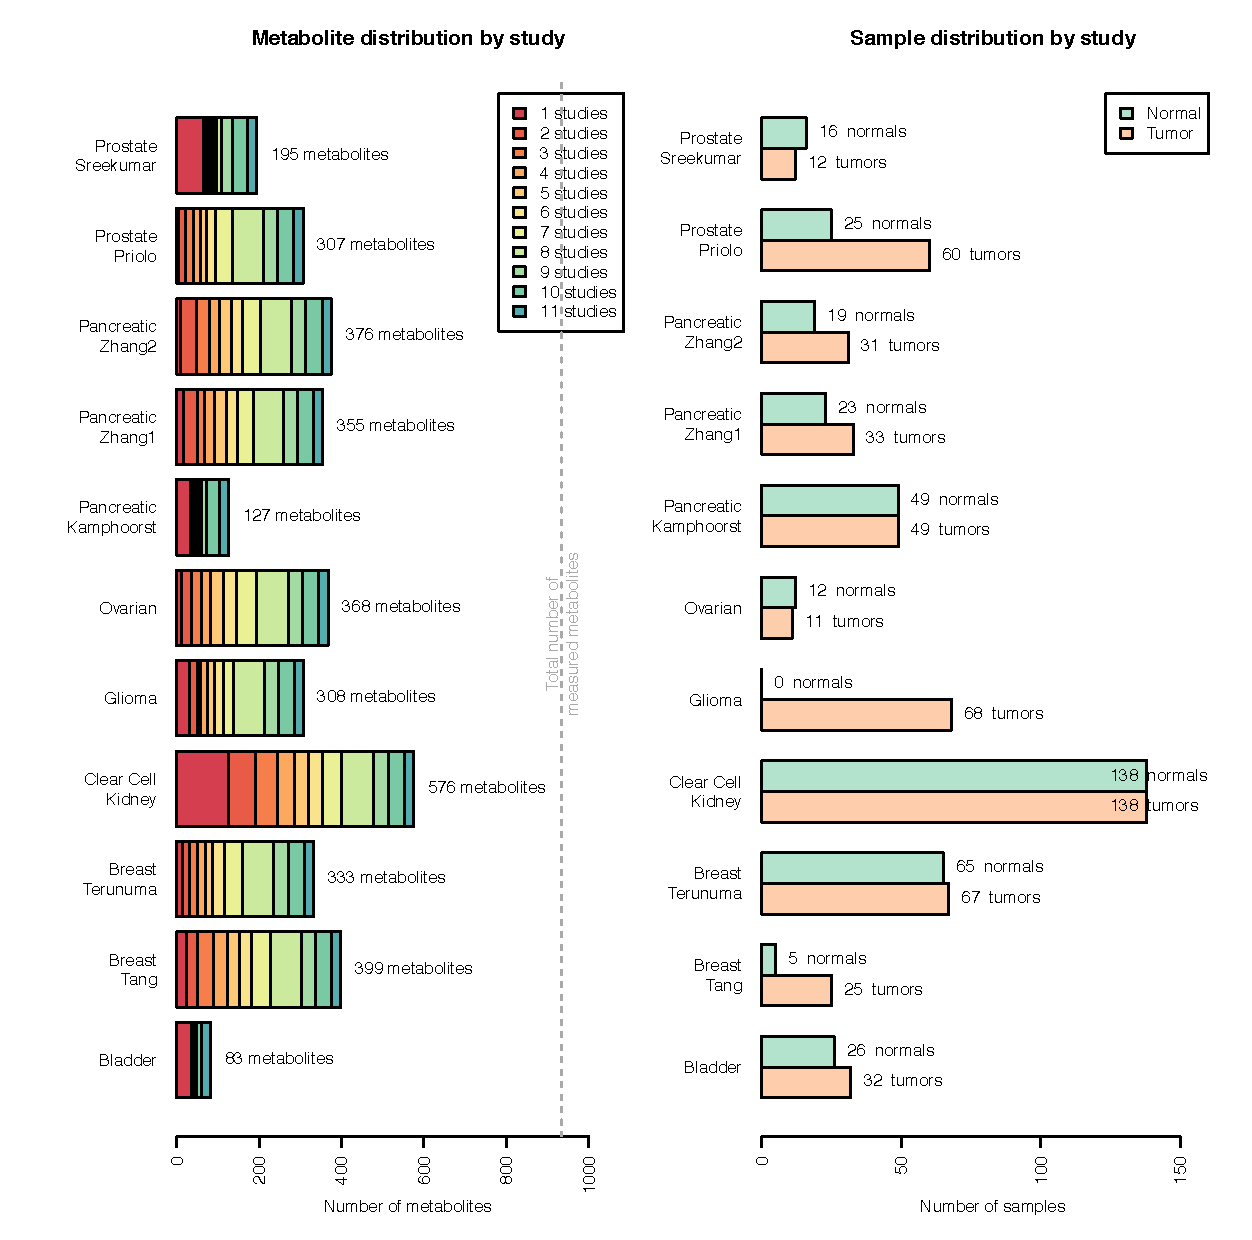
\includegraphics[scale = 0.5]{finalfigures/Figure1.pdf}
  \caption{\textbf{Metabolomics data analyzed in this study.} Data from 13 distinct metabolomics studies, examining 9 cancer types, were aggregated. Due to incomplete coverage of the metabolome, many metabolites were profiled in a small proportion of studies. The number of tumor/normal samples varied from study to study, and all but one study (gliomas) contained normal samples.}
     \label{fig:Fig1}
\end{figure}

\section{Assembly of a Cross-Cancer Compendium of Metabolomics Data}
We obtained published cancer tissue metabolomics data from thirteen datasets covering nine distinct cancer types (see Figure \ref{fig:Fig1} and Supplementary Table XX). Data from all but two cancer types was collected using mass spectrometry (colorectal and stomach cancers was collected with NMR). Three cancer types (breast, prostate, and pancreatic \cite{Hirayama2009}) were represented by at least 2 different datasets, enabling us to evaluate the consistency of findings across different studies. 

To complete a meta-analysis, we implemented a standardization pipeline (Figure \ref{fig:Fig2}) addressing two independent problems: quantatitative standardization of metabolomic measurements, and bioinformatic alignment of metabolites profiled across many studies (see Methods for detailed description). Data generated from mass spectrometry studies were in general reported as relative quantifications of metabolites (\textit{i.e.} peak intensities), rather than absolute measures of concentration. making direct comparison of the same metabolite across studies infeasible. Furthermore, across all studies, a number of metabolites were at sufficiently low abundance so as to fall outside the sensitivity of the measuring instrument, and were often imputed. Making this data amenable to quantitative analysis was essential for us, because it contained useful information indicating that the concentration of a metabolite was low (compared to samples where the concentration was within the quantifiable limits). To enable a fair comparison of metabolomics data across different studies, we implemented a common data imputation and standardization pipeline.

In addition to data standardization, a central bioinformatic challenge to our meta-analysis was the identification of metabolites profiled across multiple studies. Unlike gene expression studies, metabolomic profiling samples only a fraction of all compounds in the metabolite. More importantly,  metabolites are referred to by different synonymous names (\textit{e.g.} lactate, lactic acid, (S)-2-Hydroxypropanoate, etc.), and are often reported alongside a variety of identifiers (\textit{e.g.} KEGG IDs, HMDB IDs, Pubchem IDs). To address this issue, we developed a bioinformatic pipeline which searched for synonymous identifiers of each metabolite, and then used these synonyms to assemble a meta-dataset of all metabolomics data.

\begin{figure}[ht!]
  \centering
     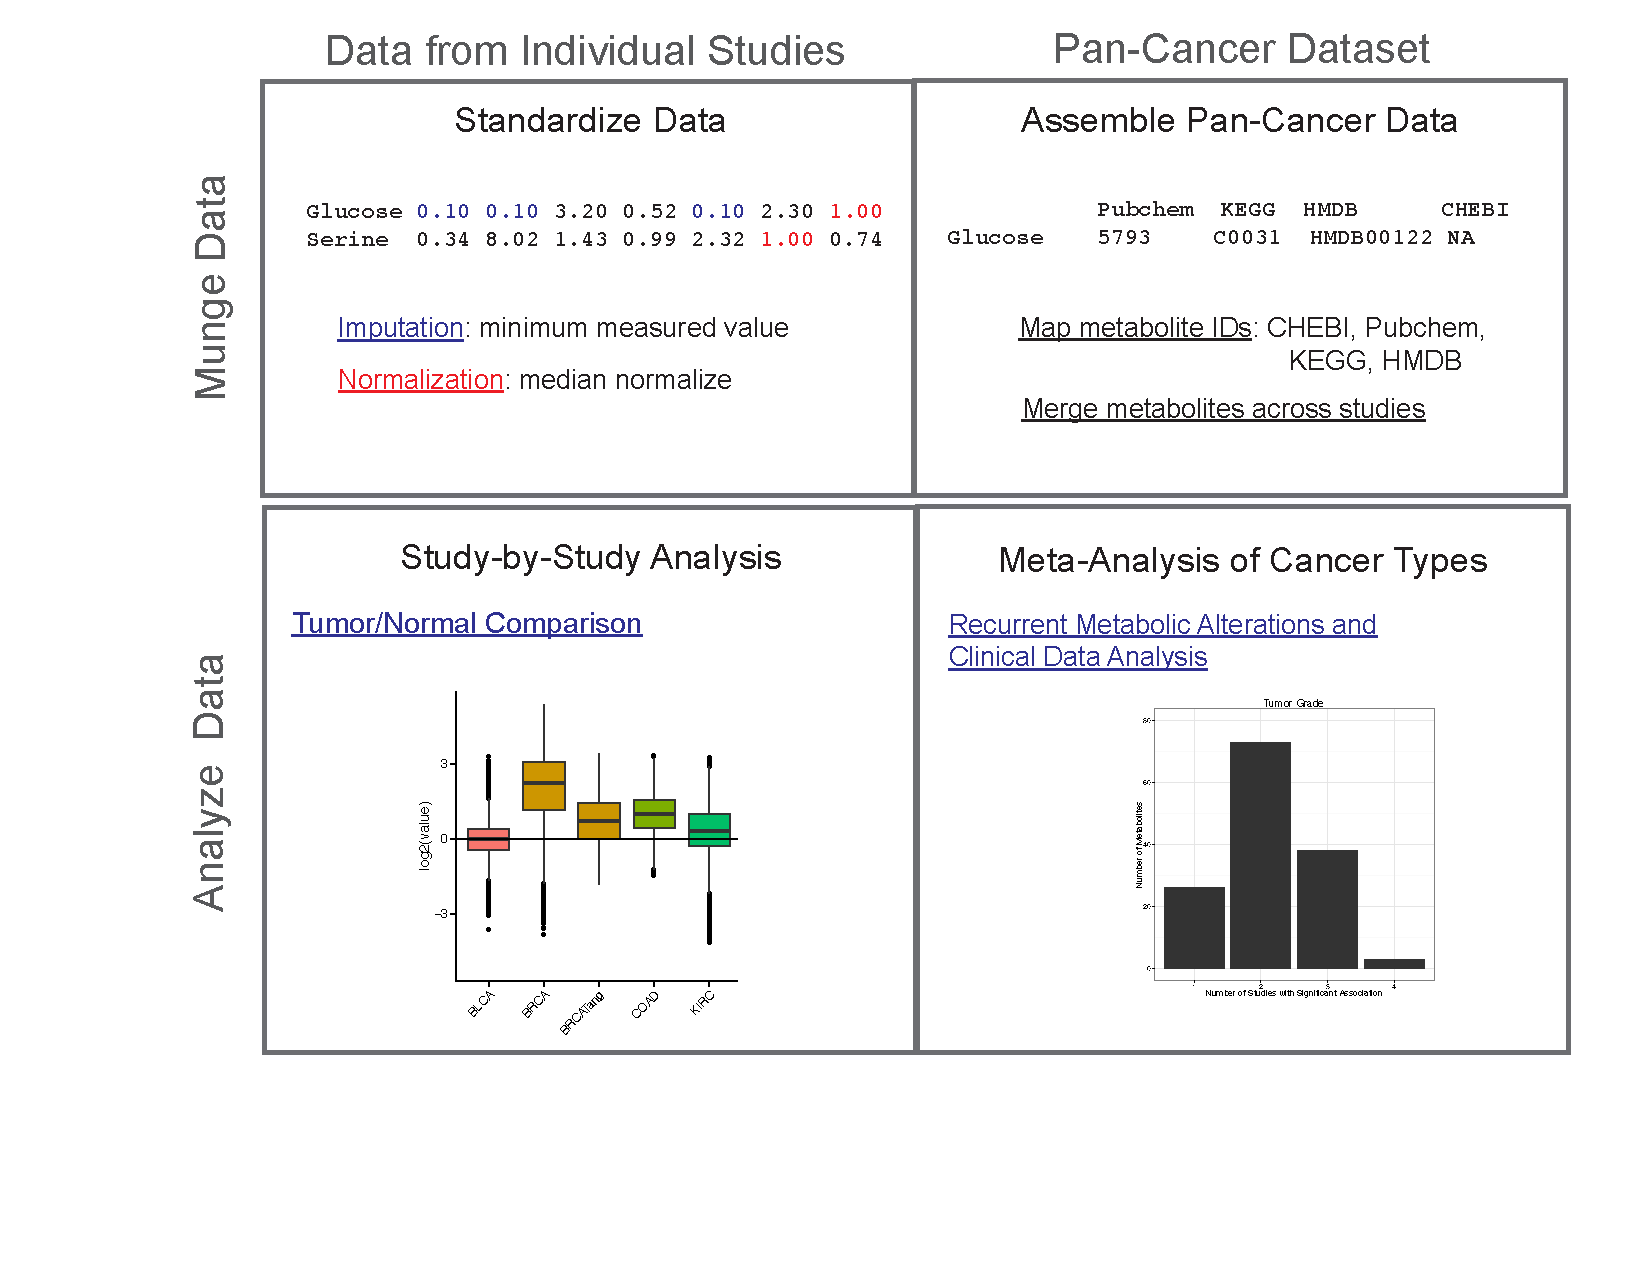
\includegraphics[scale = 0.5]{finalfigures/Figure2_workflow.pdf}
  \caption{\textbf{Data munging and analysis.} Metabolomics data from each study was imputed and standardized using a common pipeline. The resulting data was then aggregated into a meta-dataset, using a bioinformatic pipeline that identified metabolites profiled across multiple studies using metabolite identifiers such as KEGG and HMDB IDs. Analyses performed on the data included comparison to normal samples, identification of recurrent metabolic alterations, and correlation with clinical variables.}
     \label{fig:Fig2}
\end{figure}

\section{Analysis of Metabolic Variation in Tumors and Normal Tissue}

We began with a relatively simple question: how do the metabolic changes associated with transformation to cancer compare to the natural metabolic variation one might observe in normal tissue? Each tissue can be expected to have some characteristic level of fluctuation in metabolite levels. In turn, we asked if the similarity between a randomly selected pair of tumor and normal tissues is substantially greater than the similarity of two randomly chosen normal tissues. To estimate similarity, we calculated a metabolic distance between each pair of tissue samples in a study (see Methods). 

We found that the metabolic similarity of tumors and normal tissues varied greatly, in a tissue-of-origin-dependent manner (Figure \ref{fig:Fig3}). Some cancer types (including clear-cell kidney and breast cancers) were highly dissimilar from their normal tissue counterparts. At the other end of the spectrum, we observed that prostate and pancreatic tumors displayed a surprisingly small amount of variation, compared to the natural variation inherent to normal prostate and pancreatic tissue. Importantly, this effect was evident all replicate studies of the same cancer type (\textit{i.e.} both breast cancer studies showed increased variation, orange bars in Figure \ref{fig:Fig3}).

An orthogonal method for analyzing high-dimensional data, and one that is conventionally used as a first-step during analysis, is to project it onto a highly informative, low-dimensional space using performed principal components analysis (PCA).  Upon applying PCA to each dataset in our meta-analysis, we found that the majority of cancer types displayed a clear separation of tumor and normal samples. Surprisingly, however, we again found that prostate tumors and pancreatic tumors displayed poor to no separation from their respective normal samples using the first 2 principal components (see SI Figs XX-XX, evident in both prostate studies and all three of the pancreatic studies). Together with the results in Figure XX, these observations suggest that prostate and pancreatic tumors exhibit relatively small changes in the process of transformation, when compared to the natural metabolic variation evident in normal tissues.

The perplexing observation that prostate and pancreatic tumors showed relatively minor changes in metabolite abundances compared to normal tissue led us to investigate the metabolic alterations associated with tumors at higher resolution. We examined, on a study-by-study basis, which metabolites were differentially abundant between tumor and normal samples (Mann-Whitney U test, p-value < 0.05). We found the number of differentially abundant metabolites varied drastically from one cancer type to the next (Figure XX). For example, in studies of breast and clear-cell kidney tumors, we found that greater than 40 percent of metabolites showed at least a 2-fold change in abundance, whereas two independent studies of prostate cancer found that fewer than 6 percent of metabolites were differentially abundant. Importantly, because the number of tumor/normal samples were comparable for these two cancer types, the differences in differential abundance were unlikely to be statistical artifacts arising from differences in sample size.

This analysis also revealed a cancer-type-dependent trend towards unequal proportions of metabolites which increased or decreased between tumor and normal tissues. In both breast cancer studies, we found that nearly all metabolites deemed differentially abundant were at higher levels in tumor tissue, compared to normal tissue. While similar biases were evident in other studies (\textit{.e.g.} differentially abundant metabolites in pancreatic tumors tended to be at lower concentration in tumors), the effect was particularly striking for breast cancers. Although it is not possible for us to determine with certainty the source of this effect, we speculate it could arise from the disproportionate extent of data imputation for metabolites in normal breast tissue, compared to the extent of imputation in tumor tissue (Figure \ref{fig:SIFig_Imputation}).

\begin{figure}[ht!]
  \centering
     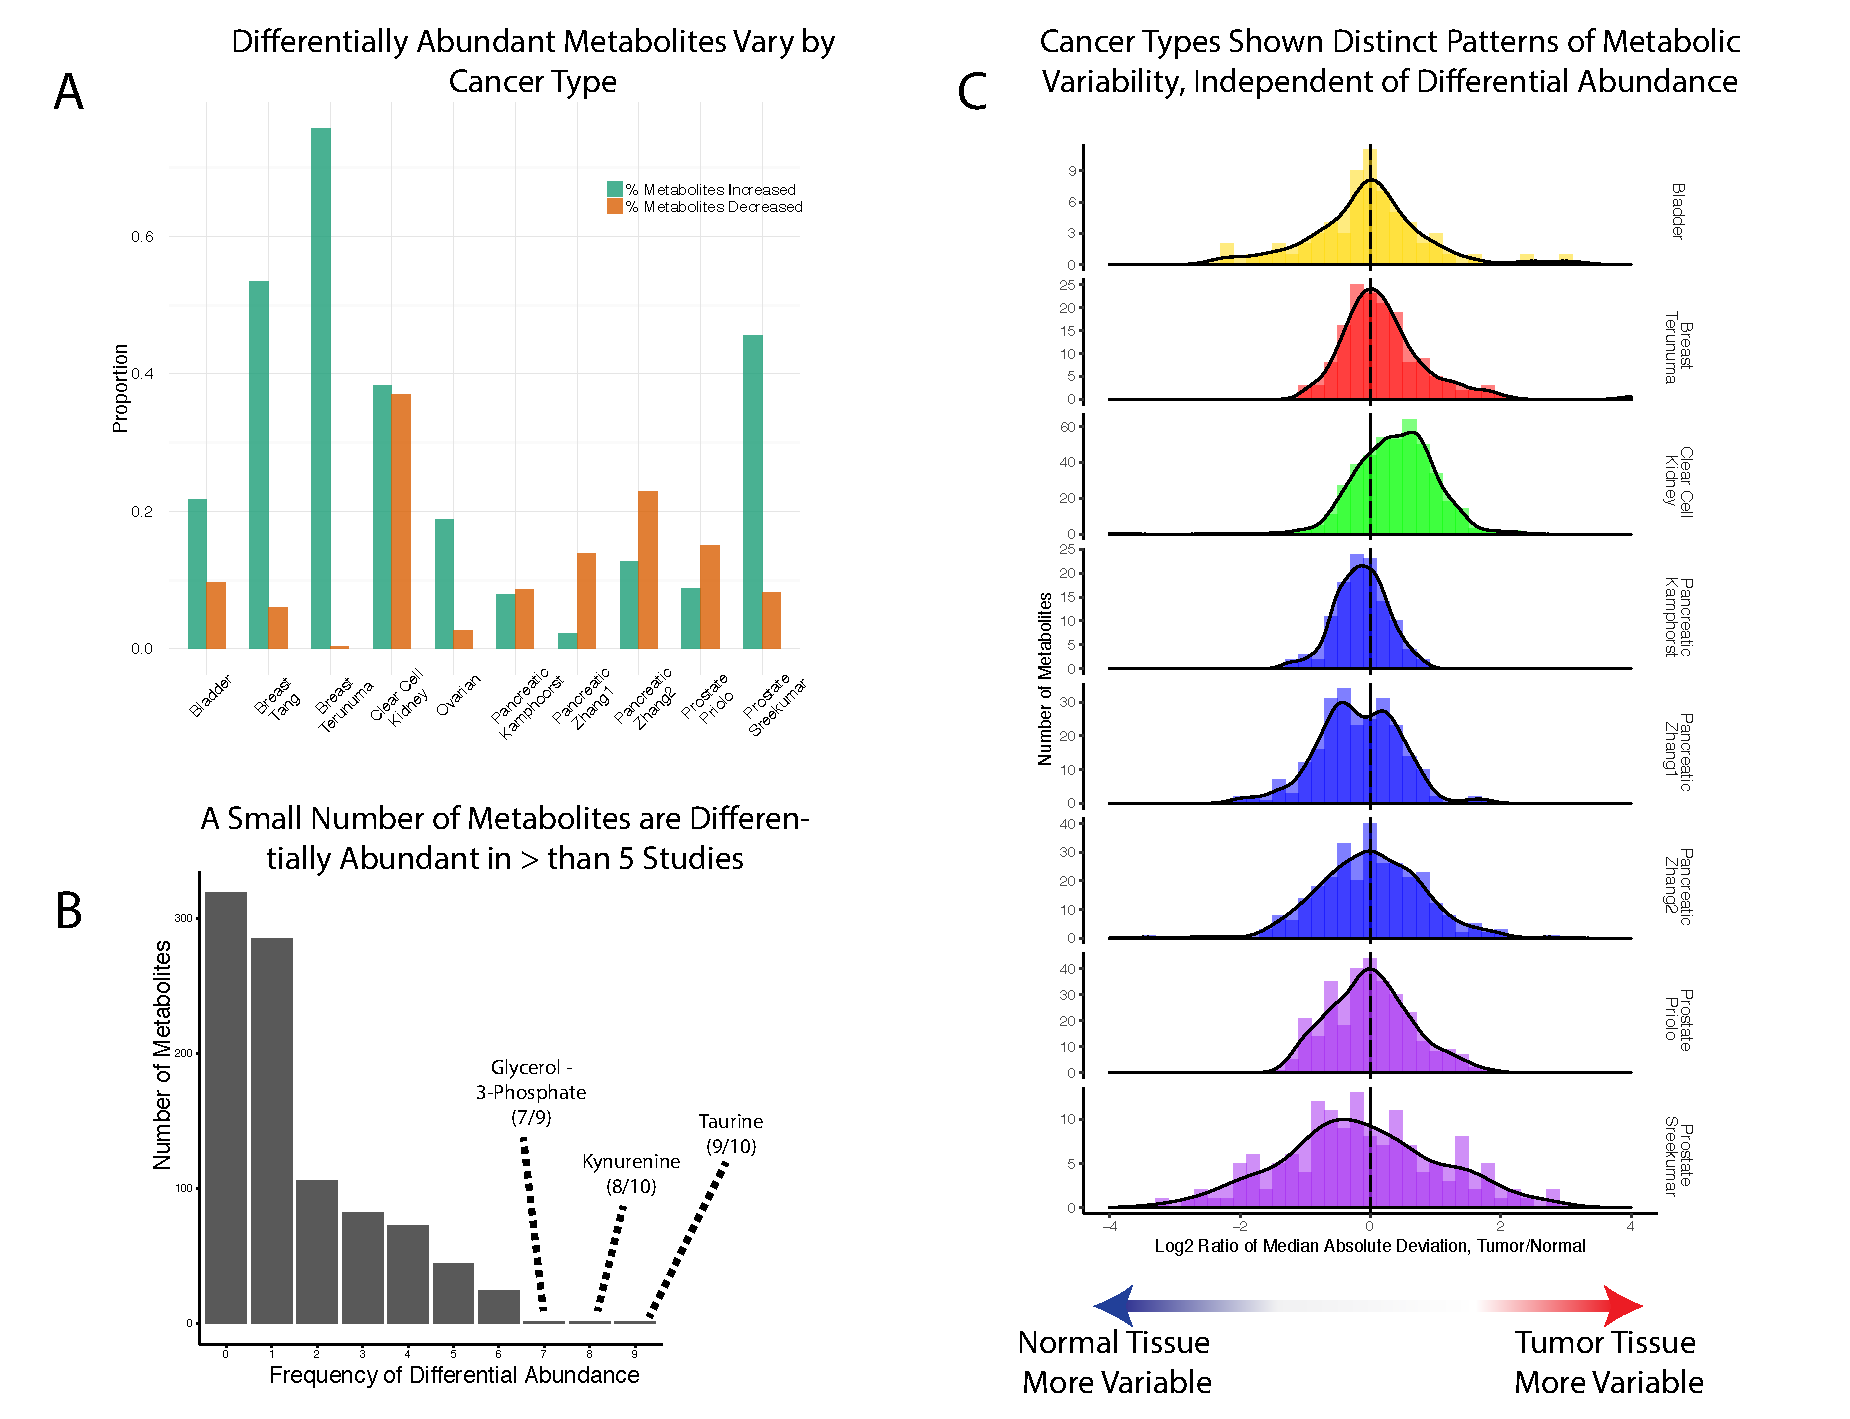
\includegraphics[scale = 0.5]{finalfigures/Figure3.pdf}
  \caption{\textbf{Tumor/Normal Comparison.} (A) Comparison of metabolic alterations in tumors to natural metabolic variation in normal tissue. By comparing the similarity of (1) randomly chosen pairs of tumor/normal tissues, to (2) randomly chosen pairs of normal tissues, we assessed the magnitude of change associated with cancerous transformation. Metabolic alterations in prostate and pancreatic tumors are small when compared with natural metabolic variation in these tissues. (B) The number of differentially abundant metabolites between tumor and normal tissues across each study varies by cancer type. Breast tumors contain the most differentially abundant metabolites, while prostate tumors contain the least. }
     \label{fig:Fig3}
\end{figure}

\section{ Common Patterns of Metabolic Alterations Across Cancers}
We were particularly interested in identifying metabolites which showed consistent patterns of increased/decreased abundance across many tumor types. The existence of such metabolites could be indicative of a cancer-type-agnostic signature of transformation. By aggregating the results of our differential abundance screen, we identified 113 metabolites differentially abundant in at least 5 studies (Supplementary Table XX). Among these, a single metabolite, taurine, was differentially abundant in ten of the twelve studies in which it was measured. Two TCA cycle metabolites (fumarate and malate), and a number of amino acids, including aspartate, asparagine, arginine, methionine, and proline, were differentially abundant in 8 studies. However, for all of these metabolites, the direction of change (\textit{i.e.} higher or lower in tumor, relative to normal) was not consistent across cancer types.

To identify metabolic alterations characteristic of transformation, we focused on metabolites which showed recurrent, consistent changes in abundance across tumor types. Two metabolites, lactate and kynurenine, were observed to increase in abundance in 8 tumor types (and decrease in abundance in zero). Three metabolites showed recurrent depletion in four distinct studies: caprate, pelargonate, and guanidoacetic acid. Both caprate and pelargonate are medium chain fatty acids, with chain lengths of ten and nine, respectively, while guanidoacetate is an intermediary metabolite of the TCA cycle. Interestingly, laurate, a medium chain fatty acid of carbon chain length 12, also showed a tendency towards recurrent downregulation (decreased in abundance in tumors in 4 studies, increased in abundance in one). 

To make greater sense of which metabolic processes may be recurrently up- or down-regulated in tumors, we used our aggregated differential abundance data to complete pathway analysis. For each study, we mapped metabolites onto KEGG pathways, and calculated an aggregate differential abundance score for each pathway (see Methods). We observed a tendency across cancers for increases in central carbon metabolism (including the KEGG pathways glycolysis/gluconeogenesis, fructose and mannose metabolism, and propanoate metaoblism), and a general down-regulation of lipid and fatty acid pathways (such as glycerolipid metabolism and fatty acid biosynthesis). Interestingly, we observed that while metabolites in the TCA cycle and oxidative phosphorylation were frequently differentially abundant, their direction of change (\textit{i.e.} higher or lower in tumors) was mixed, echoing a similar finding in a pan-cancer analysis of metabolic gene expression data \cite{Hu2013}.

\begin{figure}[ht!]
  \centering
     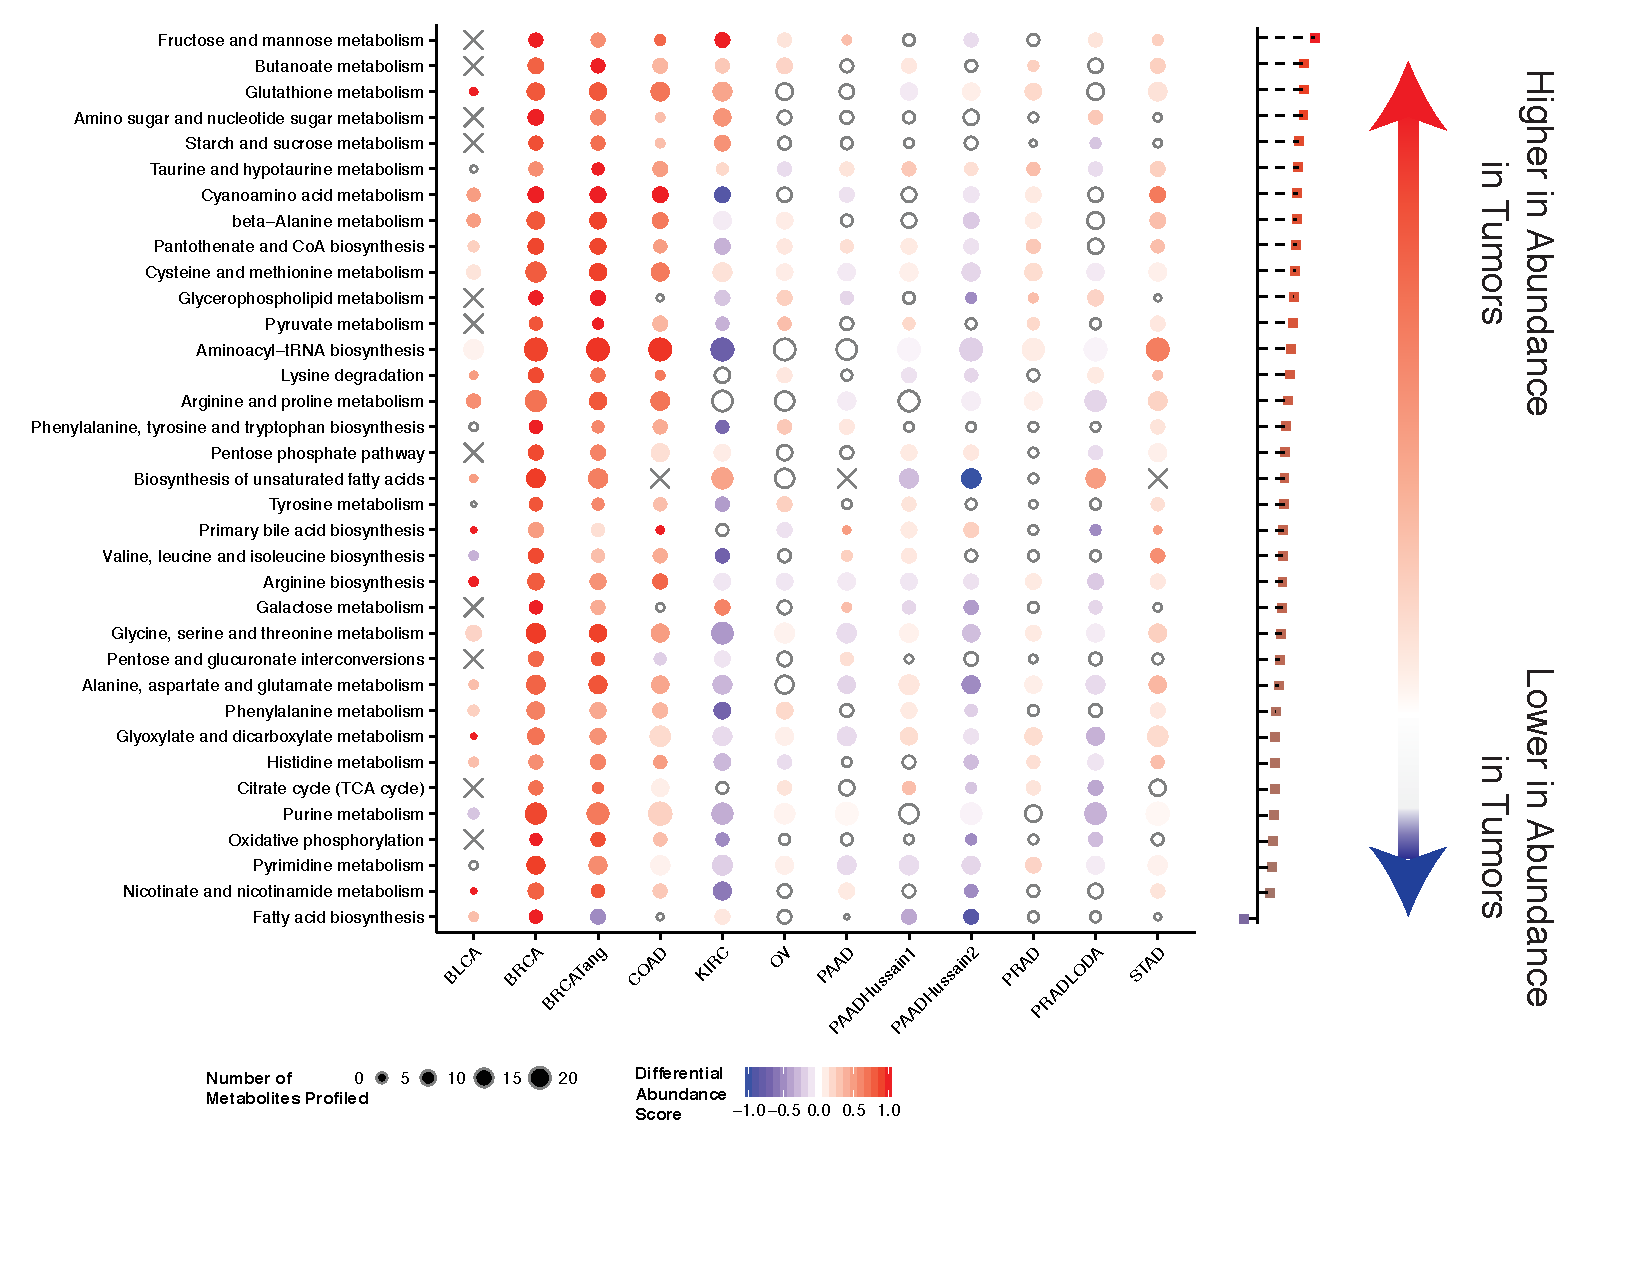
\includegraphics[scale = 0.5]{finalfigures/Figure4.pdf}
  \caption{\textbf{Recurrent metabolic alterations.} (A) Heatmap of metabolites which are differentially abundant across at least 8 different cancer studies. (B) Pathway analysis \textcolor{red}{Write more.}}
     \label{fig:Fig4}
\end{figure}

\section{Many Tumors Do Not Exhibit the Warburg Effect}
The observation that many tumors accumulate high levels of lactate, compared to normal tissue, is commonly referred to as the Warburg effect. The Warburg effect is characterized by suppression of mitochondrial oxidative phosphorylation in favor of cytosolic aerobic glycolysis, which results in the excess production and excretion of lactate. Diverting glycolytic flux towards lactate can shift cellular metabolism towards a more inefficient but also more rapid rate of ATP production, when compared to oxidative phosphorylation \cite{VanderHeiden2009}. The consequences of elevated aerobic glycolysis are often exploited in clinical imaging using fluorescent glucose for the identification of metastastic lesions \cite{CITE}.

To determine how prevalent aerobic glycolysis/the Warburg effect was in our data, we restricted our analysis to tumor samples for which matched normal tissue from the same patient was also available (347 pairs of tumor/normal tissue across 9 different cancer studies). Interestingly, we found that 84/347 (24\%) of tumor samples contained lower levels of lactate than their matched normal tissue counterpart. While most studies were enriched for tumors with increased levels of lactate, we again observed prostate tumors to be the outliers: the majority of prostate tumors showed reduced levels of lactate relative to paired adjacent normal tissue. We further confirmed whether the apparent depletion of lactate in prostate tumors (relative to normal tissue) did not arise from abberantly high levels of lactate in normal tissue (SI Figure \ref{fig:SIFig_WarburgScatter}. 

\begin{figure}[ht!]
  \centering
     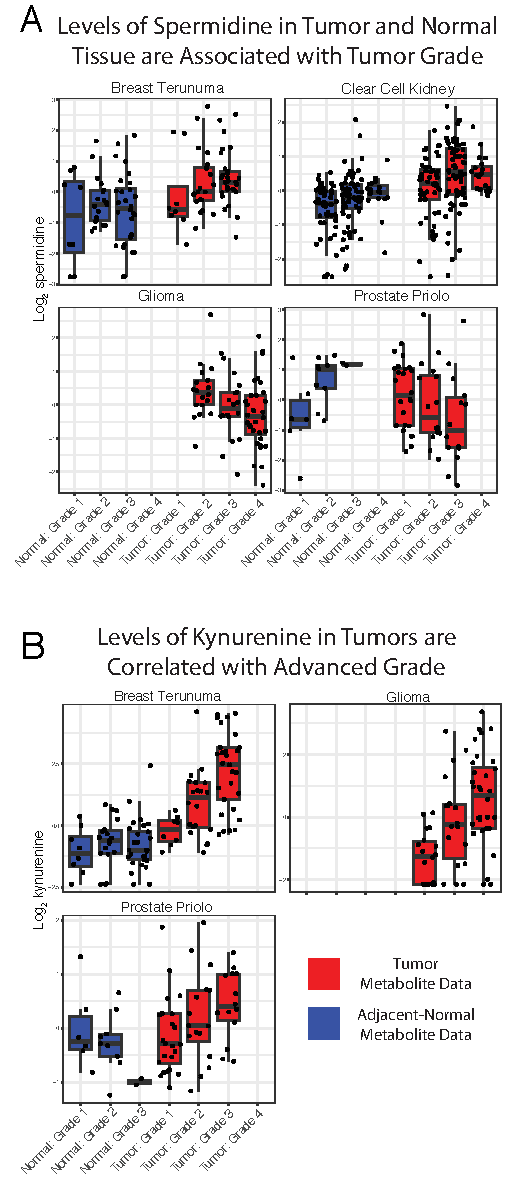
\includegraphics[scale = 0.75]{finalfigures/Figure6.pdf}
  \caption{\textbf{Many tumors do not display the Warburg effect.} (A) A quarter of tumors contained less lactate than matched normal tissue from the same patient. (B) }
     \label{fig:Fig6}
\end{figure}

Increased levels of lactate in tumor tissue are suggestive of an increase in glycolytic flux. In search of evidence to support this hypothesis, we calculated the correlation coefficient (and associated p-value) of every metabolite with levels of lactate on a study-by-study basis. Surprisingly, we observed that among glycolytic metabolites, only glucose-6-phosphate,fructose-6-phosphate, and pyruvate were positively correlated with levels of lactate in more than one study. Instead, the group of metabolites most positively correlated with lactate were urea, S-adenosylhomocysteine, and a large subset of amino acids including all three branched chain amino acids (leucine, isoleucine, valine) and two amino acids with aromatic side chains (tryptophan and phenylalanine). Taken together, these results suggest that while increased lactate levels are an indicator of increased glycolytic flux, they point further to alterations in more peripheral pathways as well.


\section{Metabolic Indicators of Tumor Progression}
The processes, including genetic and signaling events, which drive the progression of cancer to more aggressive stages are distinct from those which intitiate the tumor itself \cite{CITE}. In light of this, we examined our data for metabolic signals associated with progression of tumors to higher stage and more aggressive grade. Tumor grade is a histological measure of the extent of abnormal apperance of tumor cells. In contrast, tumor stage describes the severity of a tumor based on its size, infilitration of lymph nodes, and metastatic status. Among the 12 cancer studies which we collected in our dataset, XX had associated clinical data on tumor stage or grade. We used statistical meta-analysis techniques to identify metabolites which showed consistent changes (\textit{i.e.} consistent increase/decrease in metabolite levels with increasing tumor stage) across several cancer types. Our analyis accounted for the frequency of imputed data (see detailed description in Methods).

In total, we found 140 metabolites whose abundance were significantly correlated to tumor grade, and 60 metabolites with abundances significantly correlated to tumor stage. Filtering these results further to extract metabolites significantly associated with clinical features across many tumor types, we found 2 metabolites, erythronate and cytidine 5'-diphosphocholine, significantly associated to tumor stage in breast kidney, and ovarian cancers. We found 14 metabolites associated to tumor grade in at least 3 studies, including several amino acids (asparagine, proline, phenylalanine, leucine), 3 pyrimidines and their derivatives (thymine, uracil, and 5,6-dihydrouracil), and kynurenine. 

Among the most interesting findings was the observation that kynurenine levels were increased in tumors versus normal tissues. Kynurenine is a metabolic byproduct of the degradation of trytophan by two groups of enzymes: tryptophan dioxygenases and indoleamine 2,3-dixoygenases. Binding of kynurenine to aryl hydrocarbon receptors (AHRs) and suppress the activity of T-effector cells, as well as indirectly activating regulatory pro-tumorigenic T cells. Kynurenine was unique in our study because it was found to be elevated in the majority of tissues, and it was also found to be positively correlated to tumor grade in 4 different studies (2 different prostate cancer studies, as well as breast cancers and gliomas). Together, these findings point to a critical role for kynurenine in the metabolism of tumors.

\begin{figure}[ht!]
  \centering
     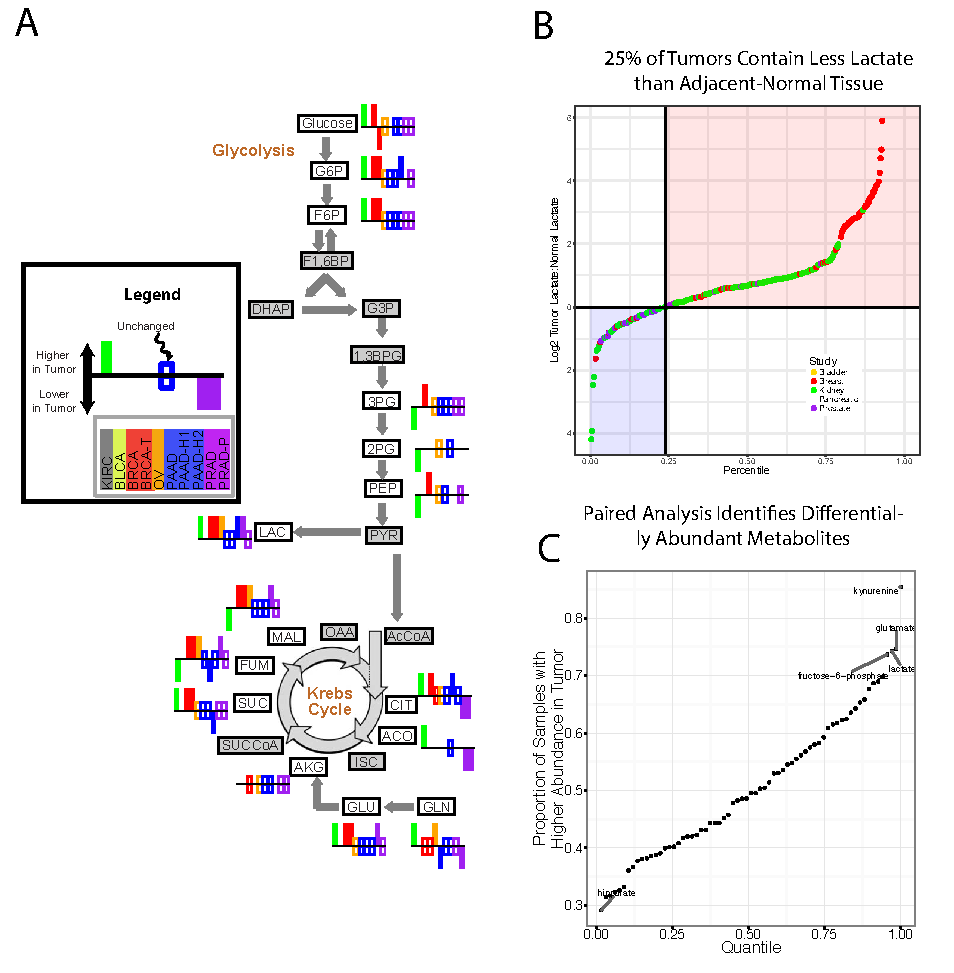
\includegraphics[scale = 0.5]{finalfigures/Figure5.pdf}
  \caption{\textbf{Metabolic correlation with tumor progression.} (A) and (B) Relatively few metabolites correlate with tumor stage and grade across multiple cancer types. (C) Kynurenine is significantly associated with tumor grade across three different cancer types (breast, gliomas, and  prostate cancers.}
     \label{fig:Fig5}
\end{figure}


\section{Discussion}

umors must bear the metabolic challenges faced by the tissue they arise, from the frequent osmotic stress inherent to the filtration performed by kidney cells to the xenobiotic stress endured by cells of the liver. Thus, it should come as no surprise that tumors  vary substantially in how their metabolic phenotype. In this study, we examined in detail the extent of this variation across nine cancer types. While we observed that some tumors (\textit{e.g.} of the prostate) appear to show comparatively minor metabolic alterations compared to other cancer types, we also found metabolic alterations common to the majority of cancer types (\textit{e.g.} the increase in abundance of lactate and kynurenine). 

Our approach to the assembly and alignment of several metabolomics studies relied on several computational pipelines which we expect to serve as a benchmark for future work. As described in detail earlier and in the Methods, the majority of data compiled here was reported in terms of (dimensinoaless) relative abundances, rather than absolute concentrations. To make data across studies comparable, we implemented a computational pipeline which assured, where possible, common standards for data imputation and standardization. We also implemented a bioinformatic pipeline to ``align'' metabolites identified by distinct metabolite identifiers, the code for which is included as a supplementary file (SI File XX). To compare results across studies, we relied heavily on non-parametric statistics, and used changes relative to normal tissue as the fundamental unit of comparison. 

Challenges arising from the assembly: aligning metabolites, common imputation and standardization, 

Value of the data to the community at large: resource for validating observations, and for future inquiries into metabolism (co-variation of metabolites?)



Perhaps the first challenge we encountered during data collection was the difficulty of ``aligning'' a metabolite which had been profiled in more than one study, but was labeled with a distinct name (\textit{e.g.} lactate, lactic acid, L-lactate, (S)-lactate)). Typically, metadata regarding the chemical identity of metabolites (\textit{i.e.} KEGG IDs, PubChem IDs) was included in studies, but this metadata was universally incomplete. In most cases, a study would include either a KEGG ID or an HMDB ID for a metabolite, but not both. This made the task of finding common metabolites across studies exceptionally challenging. To overcome this challenge, we developed a bioinformatic method for assembling a list of consistent metabolite identifiers for each metabolite profiled in each study.

A second challenge arose from the large amount of incomplete data. 

Third, nearly all of the data in the meta-analysis (with the exception of the COAD/STAD data) 

The final, and perhaps most challenging, complication of our data was that, because of incomplete coverage of the metabolome, very few metabolites were profiled across more than a small number of studies. This challenge became increasingly important to address when attempting to cluster the metabolomics data across many tumor types, because the number of metabolites concordantly sampled varied from one pair of studies to the next. As a result, the dimensionality of the data varied from one pair of samples to the next, making calculating distances challenging. We proposed a non-parametric clustering approach which handled incongruous dimensionality, and showed that it identified an outlying cluster of ccRCC tumors distinguished by elevated levels of dipeptides.


\section{Methods}

\subsection{Data Imputation and Standardization}
For data which was already imputed and standardized (including the BLCA, KIRC, BRCA, BRCATang, OV, PAADHussain1, PAADHussain2, PRADLODA studies), we used the data as reported by the original authors. For five studies (COAD,LGG,PAAD,PRAD,and STAD) for which no imputation was completed, we applied the following imputation and standardization procedure. For each metabolite, imputed values were set equal to the minimum measured abundance of that metabolite. Then, all measurements of the metabolite were median normalized. 

\subsection{Metabolite ID Mapping}
\textcolor{red}{Augustin please fill in}

\subsection{Differential Abundance Tests}
Differential abundance was calculated using the ratio of the average abundance of a metabolite in tumor tissue, to the average abundance of a metabolite in normal tissue. Statistical significance was assessed using non-paramatric Mann-Whitney U-tests.

\subsection{Pathway Differential Abundance Score}
The differential abundance score for a pathway was defined as

\begin{align*}
DA = \frac{I - D}{S}
\end{align*}

\noindent where $I$ is the number of measured metabolites in a pathway which increased in abundance relative to normal tissue, $D$ is the number which decreased, and $S$ is the total number of measured metabolites. A $DA$ score of 1 indicates that all metabolites increased in abundance, whereas a score of -1 indicates that all metabolites decreased in abundance, relative to normal tissue.

\subsection{Metabolomics Data Acquisition and Normalization}
Metabolomics data from prior, published work was obtained either through the corresponding journal, or by contacting the corresponding author. The data for all studies except COAD and STAD was reported in relative abundances, \textit{i.e.} the abundance of a metabolite $i$ in sample $j$ could only be compared to other values of metabolite $i$ in different samples from the same study. For COAD and STAD, absolute abundances were reported.

Because metabolomics data does not necessarily obey a known distribution, we applied minimal normalization techniques in order to make data minimally comparable across all studies. For each metabolite in a study, we calculated the median abundance, and normalized by this abundance. Given the unknown distribution of the data in our study, we used only non-parametric statistical tests (which are independent of data distribution) to assess changes in metabolite abundance.

\subsection{Correlation with Lactate Levels}
Within each study which profiled lactate abundance, spearman correlations and associated p-values were calculated between the levels of all profiled metabolites and lactate. P-values across all studies were combined using Fisher's method and a chi-squared test was applied to determine statistical significance \cite{Whitlock2005}. P-values from the chi-squared test were corrected using the Benjamini-Hochberg procedure.

\subsection{Association with Stage and Grade}
Different statistical tests were applied to identify correlation between metabolites and clinical features depending on the level of censoring in the data. If there is less than 20\% censoring within the tested set, the Jonckheere-Terpstra test (a non-parametric test which uses permutations to calculate the p-value) was used to examine ordered differences among classes . If there are more than 20\% but less than 80\% censored data, an exact log-rank trend test is used for interval (left) censored data. Both tests assume a metabolite should increase/decrease monotonically with stage/grade.  If there is more than 80\% censoring no test is used, and the metabolite is ignored. To summarize the tests across cohorts I use Fisher’s method to combine p-values. Note that resulting combined p-value is parametric. 

Since we are interested in finding associations of a common sign (\textit{e.g.} consistently positive correlation across multiple studies), one-sided p-values are calculated first, aggregate into a combined p-value using Fisher's method \cite{Whitlock2005}, and then transformed to two-sided combined p-value.

\bibliographystyle{plain}
\bibliography{panmet}

\beginsupplement
\newpage

\begin{table}
\centering
\begin{tabular}{ c c c c }
  \textbf{Study Name} & \textbf{Cancer Type} & Data Type & \textbf{Reference}  \\
  \hline
  BLCA & Bladder & Mass Spectrometry & \cite{Putluri2011} \\
  BRCA & Breast & Mass Spectrometry & \cite{Terunuma2014} \\
  BRCATang & Breast & Mass Spectrometry & \cite{Tang2014} \\
  COAD & Colorectal & NMR & \cite{Hirayama2009} \\
  KIRC & Clear-cell Renal Cell & Mass Spectrometry & \cite{Hakimi2015} \\
  LGG & Glioma & Mass Spectrometry & \cite{Chinnaiyan2012} \\
  OV & Ovarian & Mass Spectrometry & \cite{Fong2011} \\
  PAAD & Pancreas & Mass Spectrometry & \cite{Kamphorst2015} \\
  PAADHussain1 & Pancreas & Mass Spectrometry & \cite{Zhang2013} \\
  PAADHussain2 & Pancreas & Mass Spectrometry & \cite{Zhang2013} \\
  PRAD & Prostate & Mass Spectrometry & \cite{Sreekumar2009} \\
  PRADLODA & Prostate & Mass Spectrometry & \cite{Priolo2014} \\
  STAD & Stomach & NMR & \cite{Hirayama2009}
\end{tabular}
\caption{Summary of the published cancer tissue metabolomics studies examined in this work.}
\label{table:SITab_Studies}
\end{table}

\begin{figure}[ht!]
  \centering
     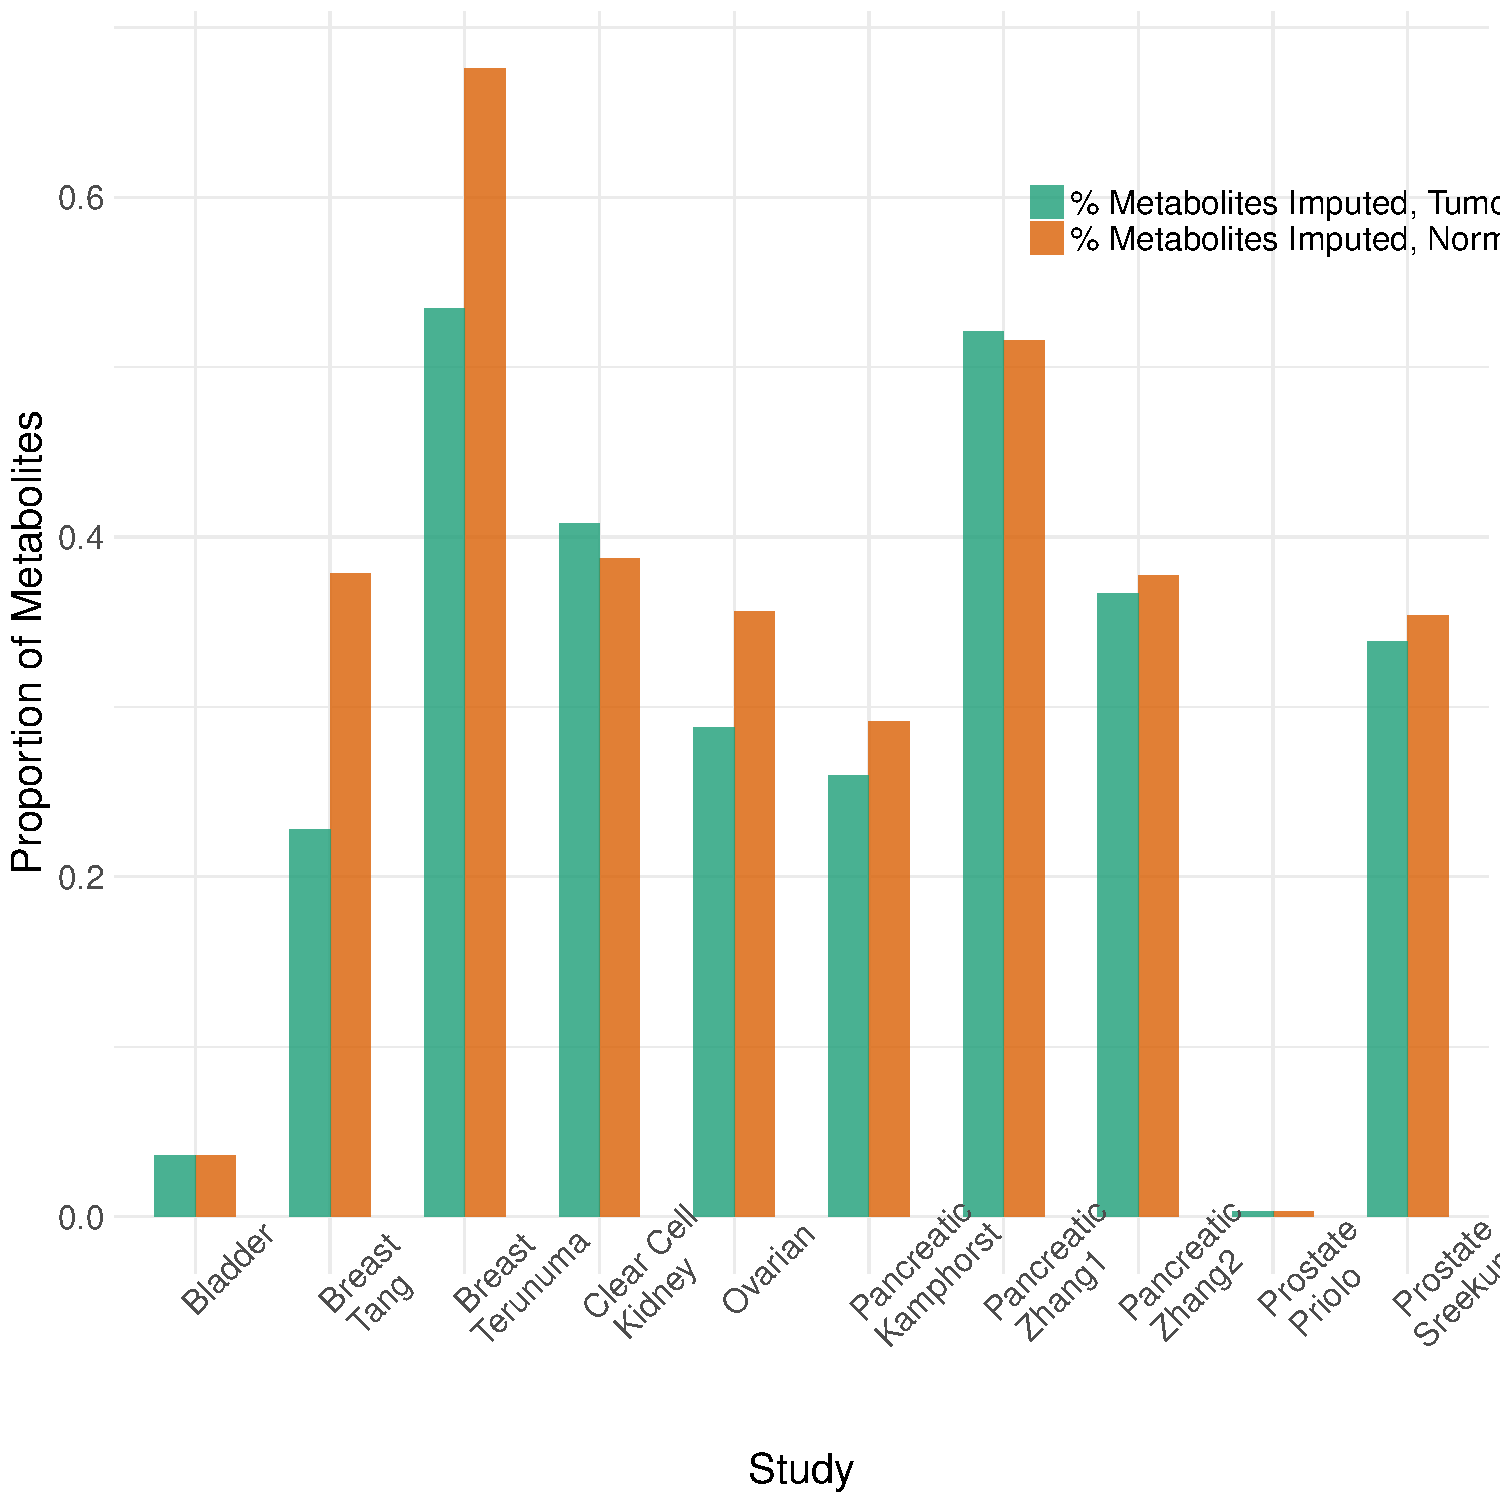
\includegraphics[scale = .6]{finalfigures/imput_barplot.pdf}
  \caption{For each study, we calculated the proportion of metabolites with greater than 20\% imputation in tumor samples. The calculation was repeated separately for normal samples. The two breast studies are exceptional because of the incongruent level of imputation between normal and tumor samples: far more metabolites are heavily imputed in normal breast samples, compared breast tumor samples. }
     \label{fig:SIFig_Imputation}
\end{figure}

\begin{figure}[ht!]
  \centering
     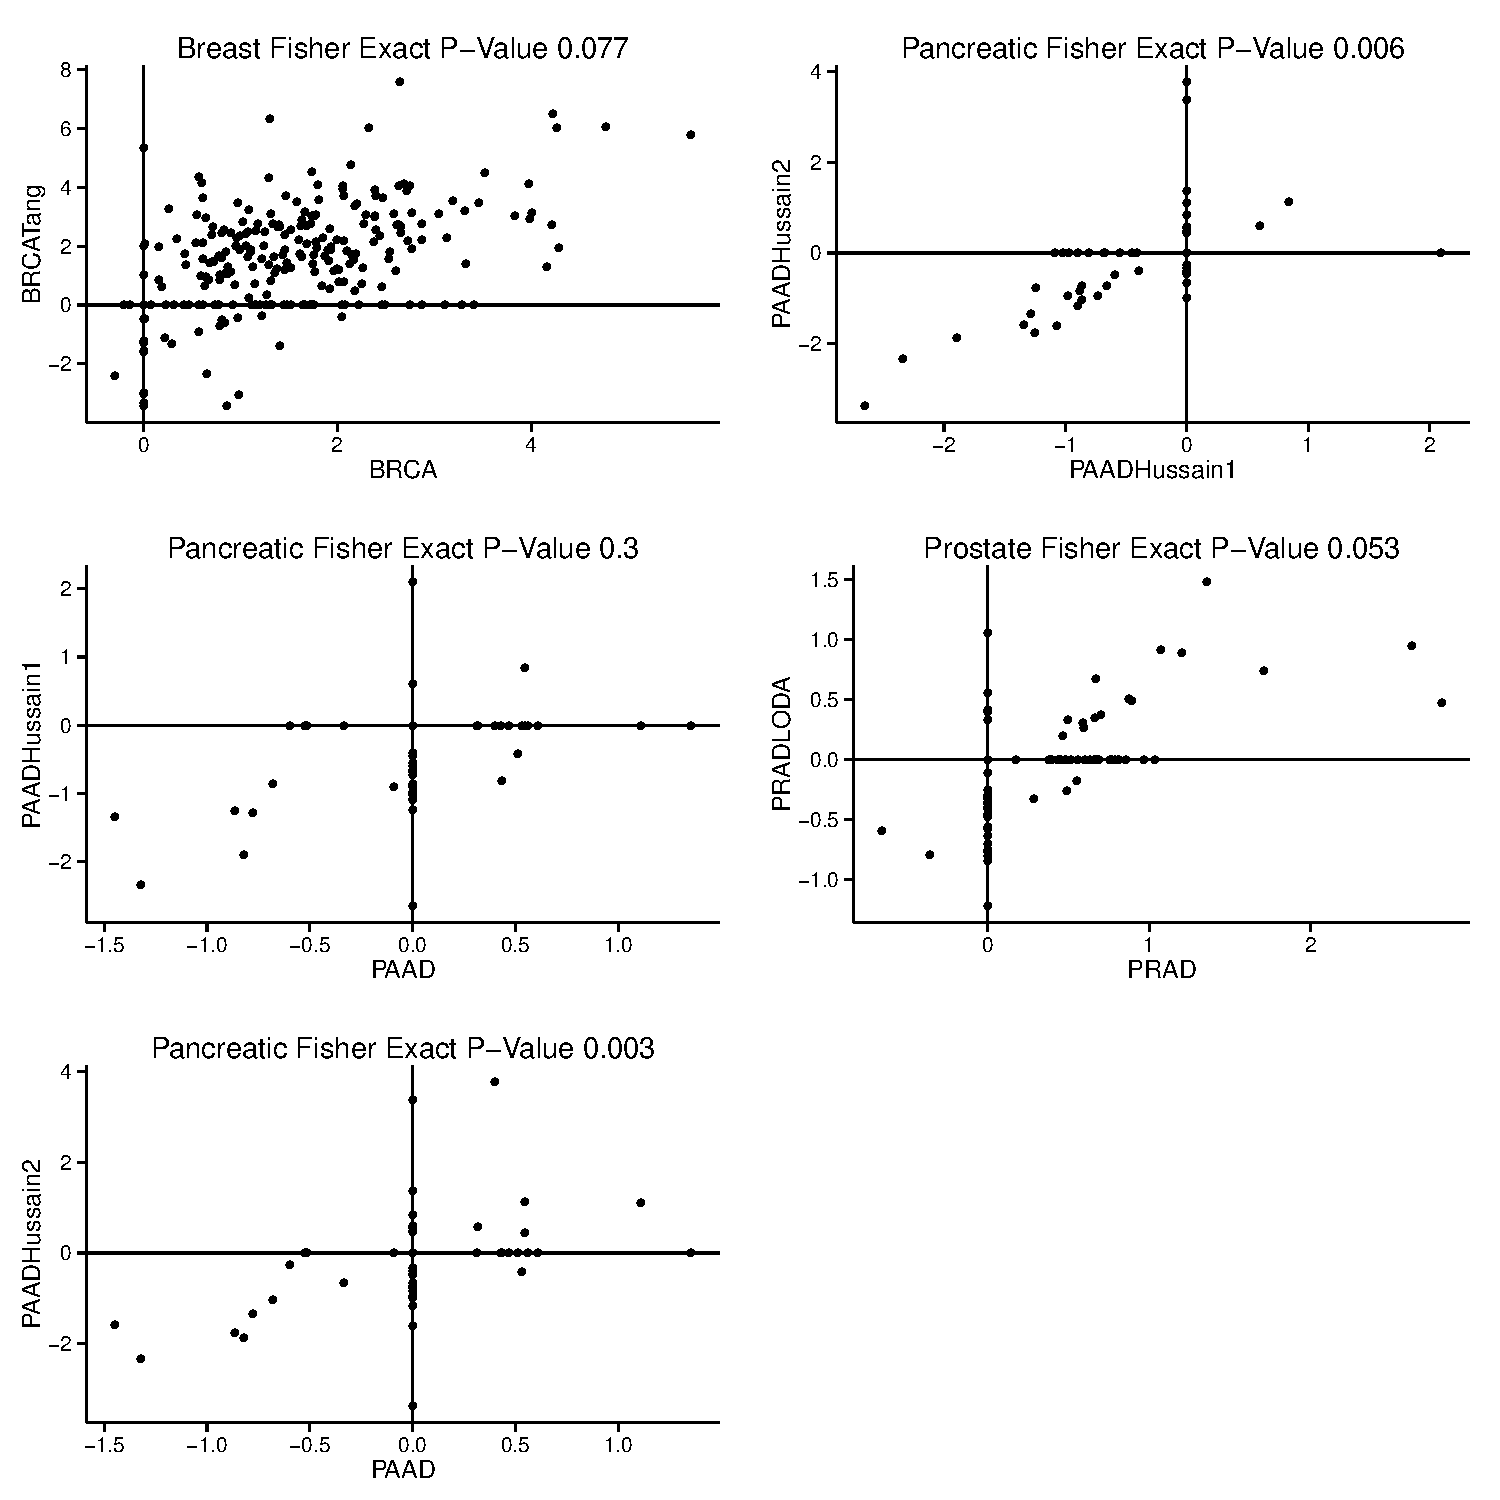
\includegraphics[scale = .6]{finalfigures/sametissue.pdf}
  \caption{Insert caption.}
     \label{fig:SIFig_SameTissue}
\end{figure}

\begin{figure}[ht!]
  \centering
     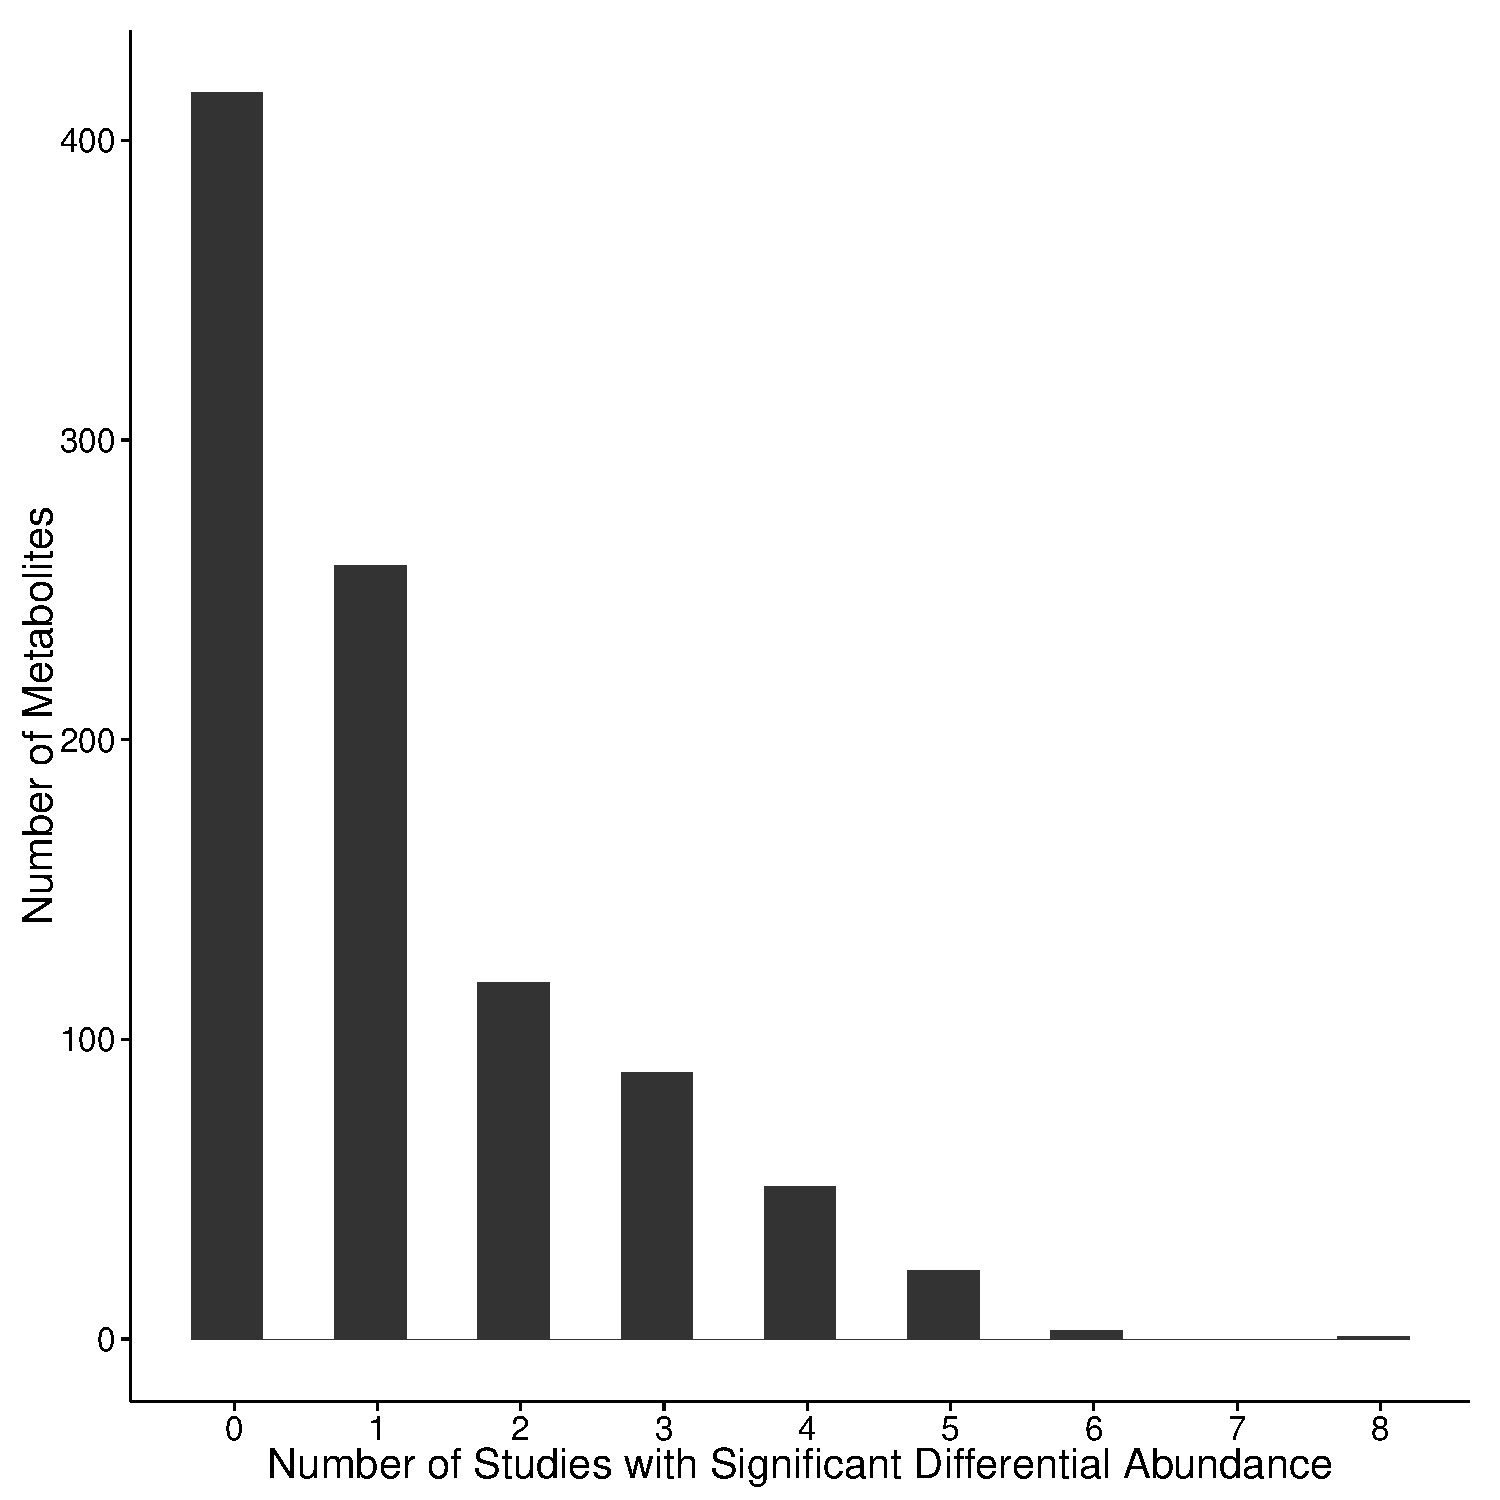
\includegraphics[scale = .6]{finalfigures/Histogram_NumDiffAbundant.pdf}
  \caption{Insert caption.}
     \label{fig:SIFig_HistogramDiffAbundance}
\end{figure}
 

\begin{figure}[ht!]
  \centering
     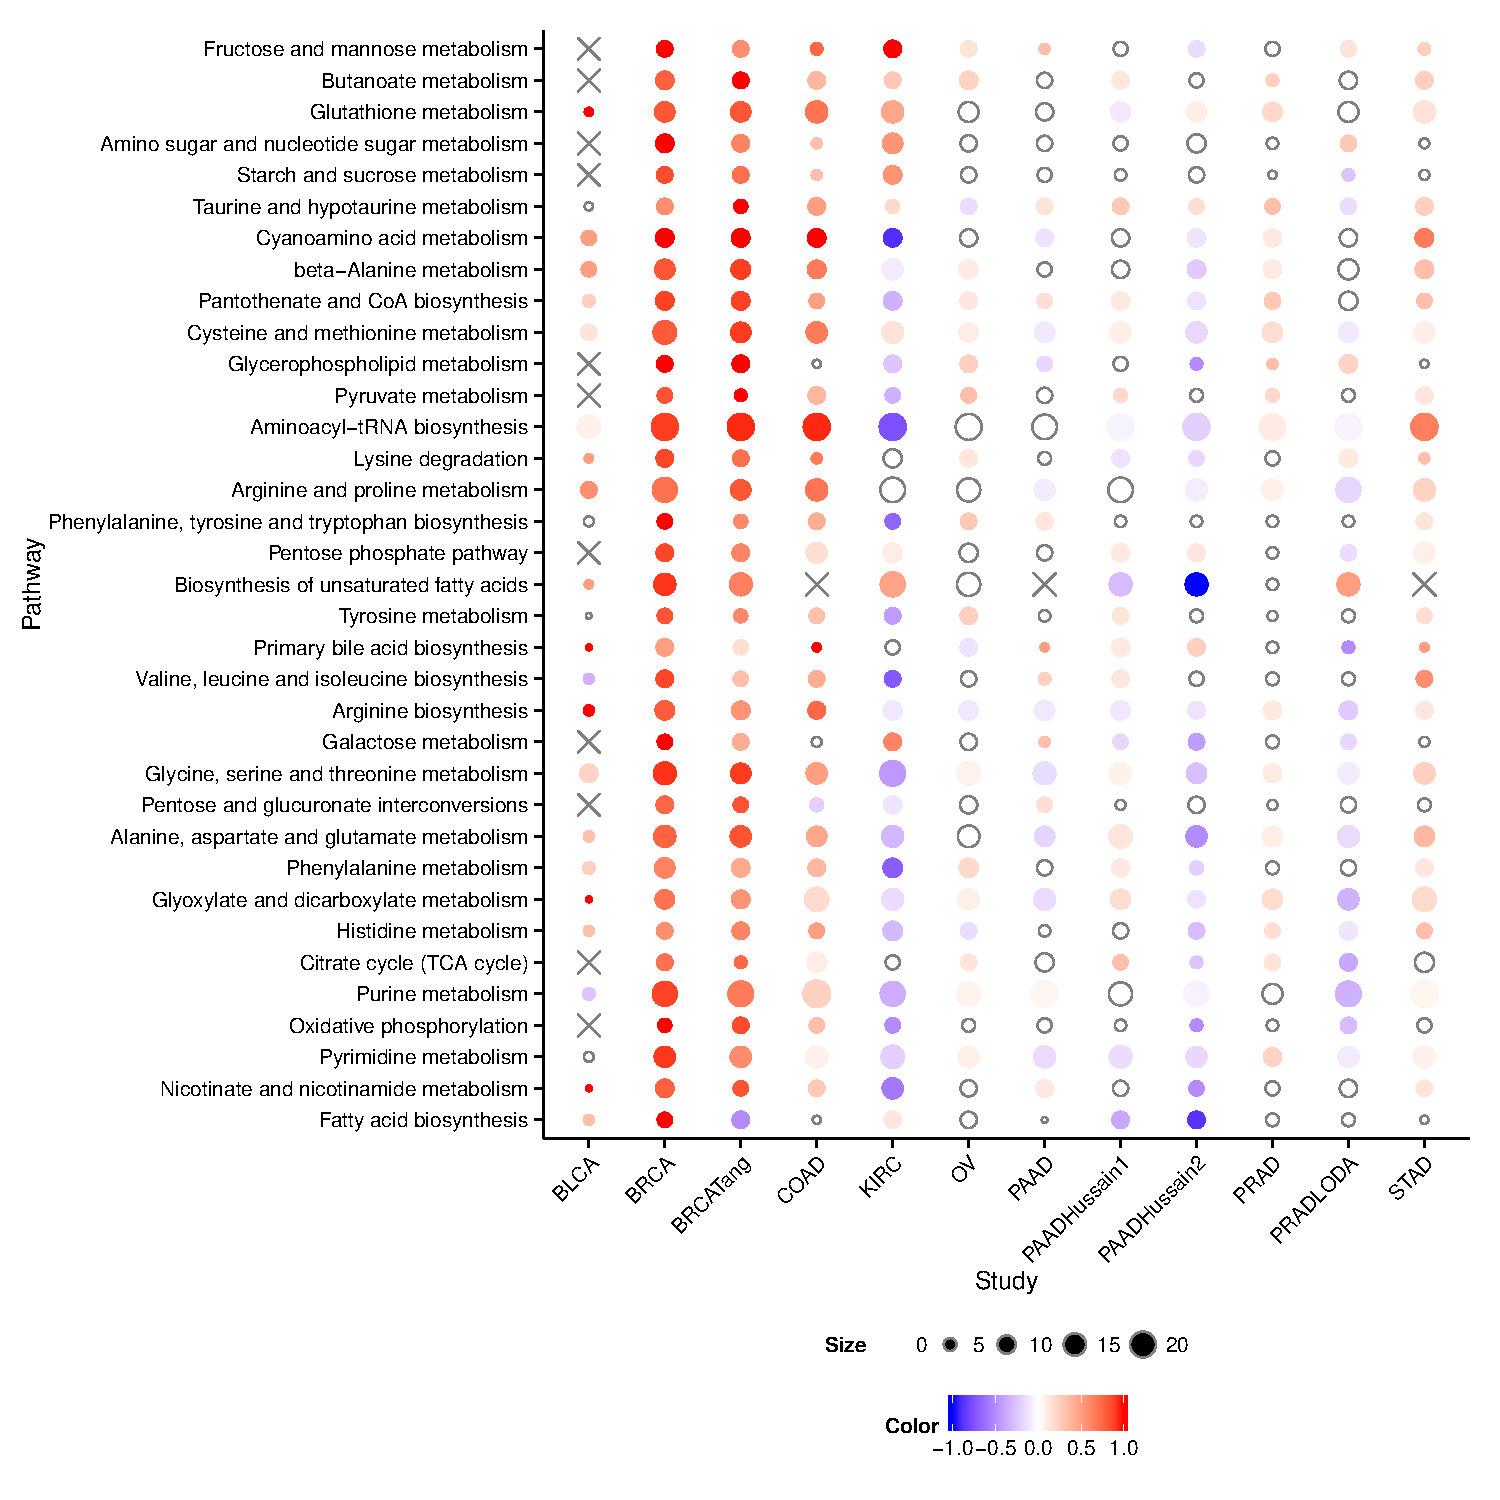
\includegraphics[scale = .6]{finalfigures/pathway_heatmap.pdf}
  \caption{Insert caption.}
     \label{fig:SIFig_PathwayHeatmap}
\end{figure}

\begin{figure}[ht!]
  \centering
     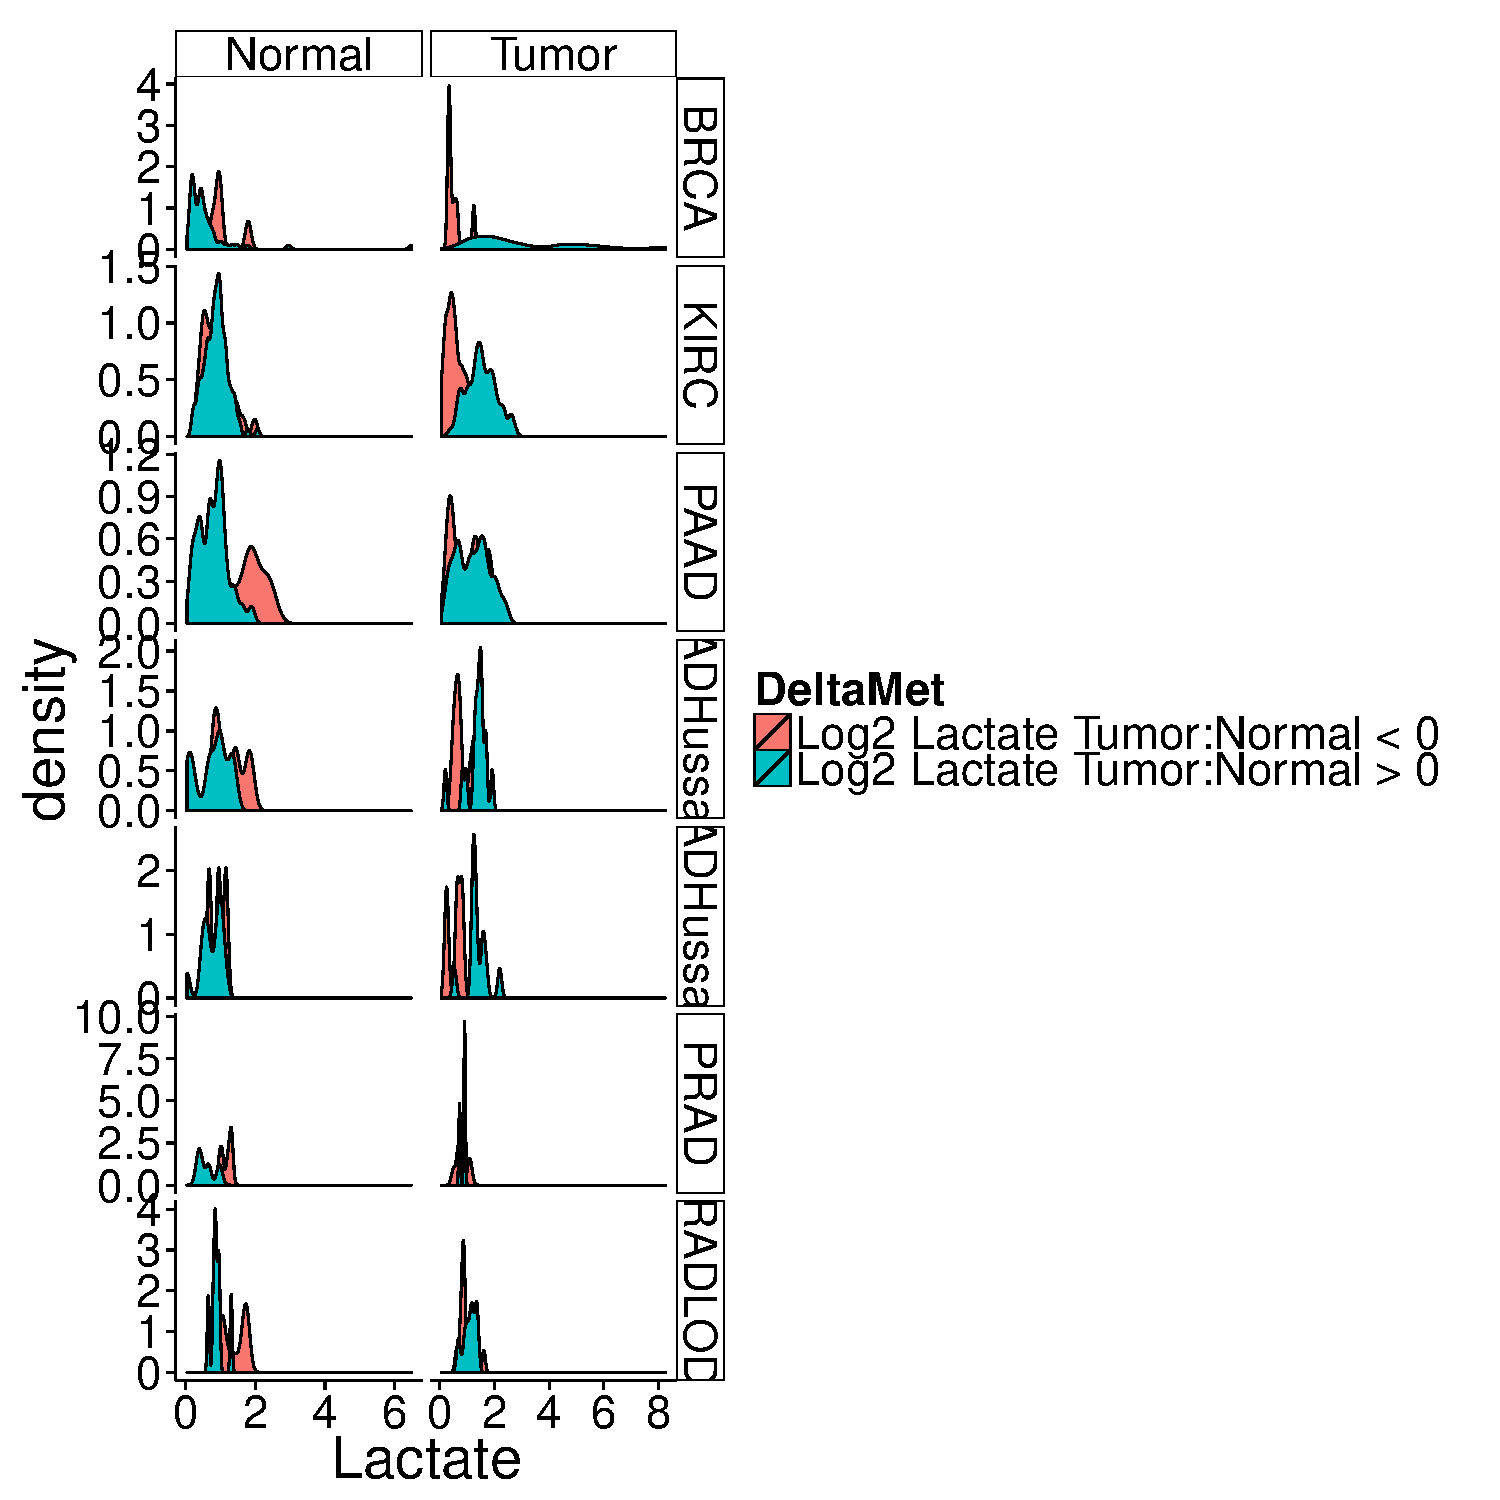
\includegraphics[scale = .6]{finalfigures/warburg_source.pdf}
  \caption{Insert caption.}
     \label{fig:SIFig_WarburgSource}
\end{figure}

\begin{figure}[ht!]
  \centering
     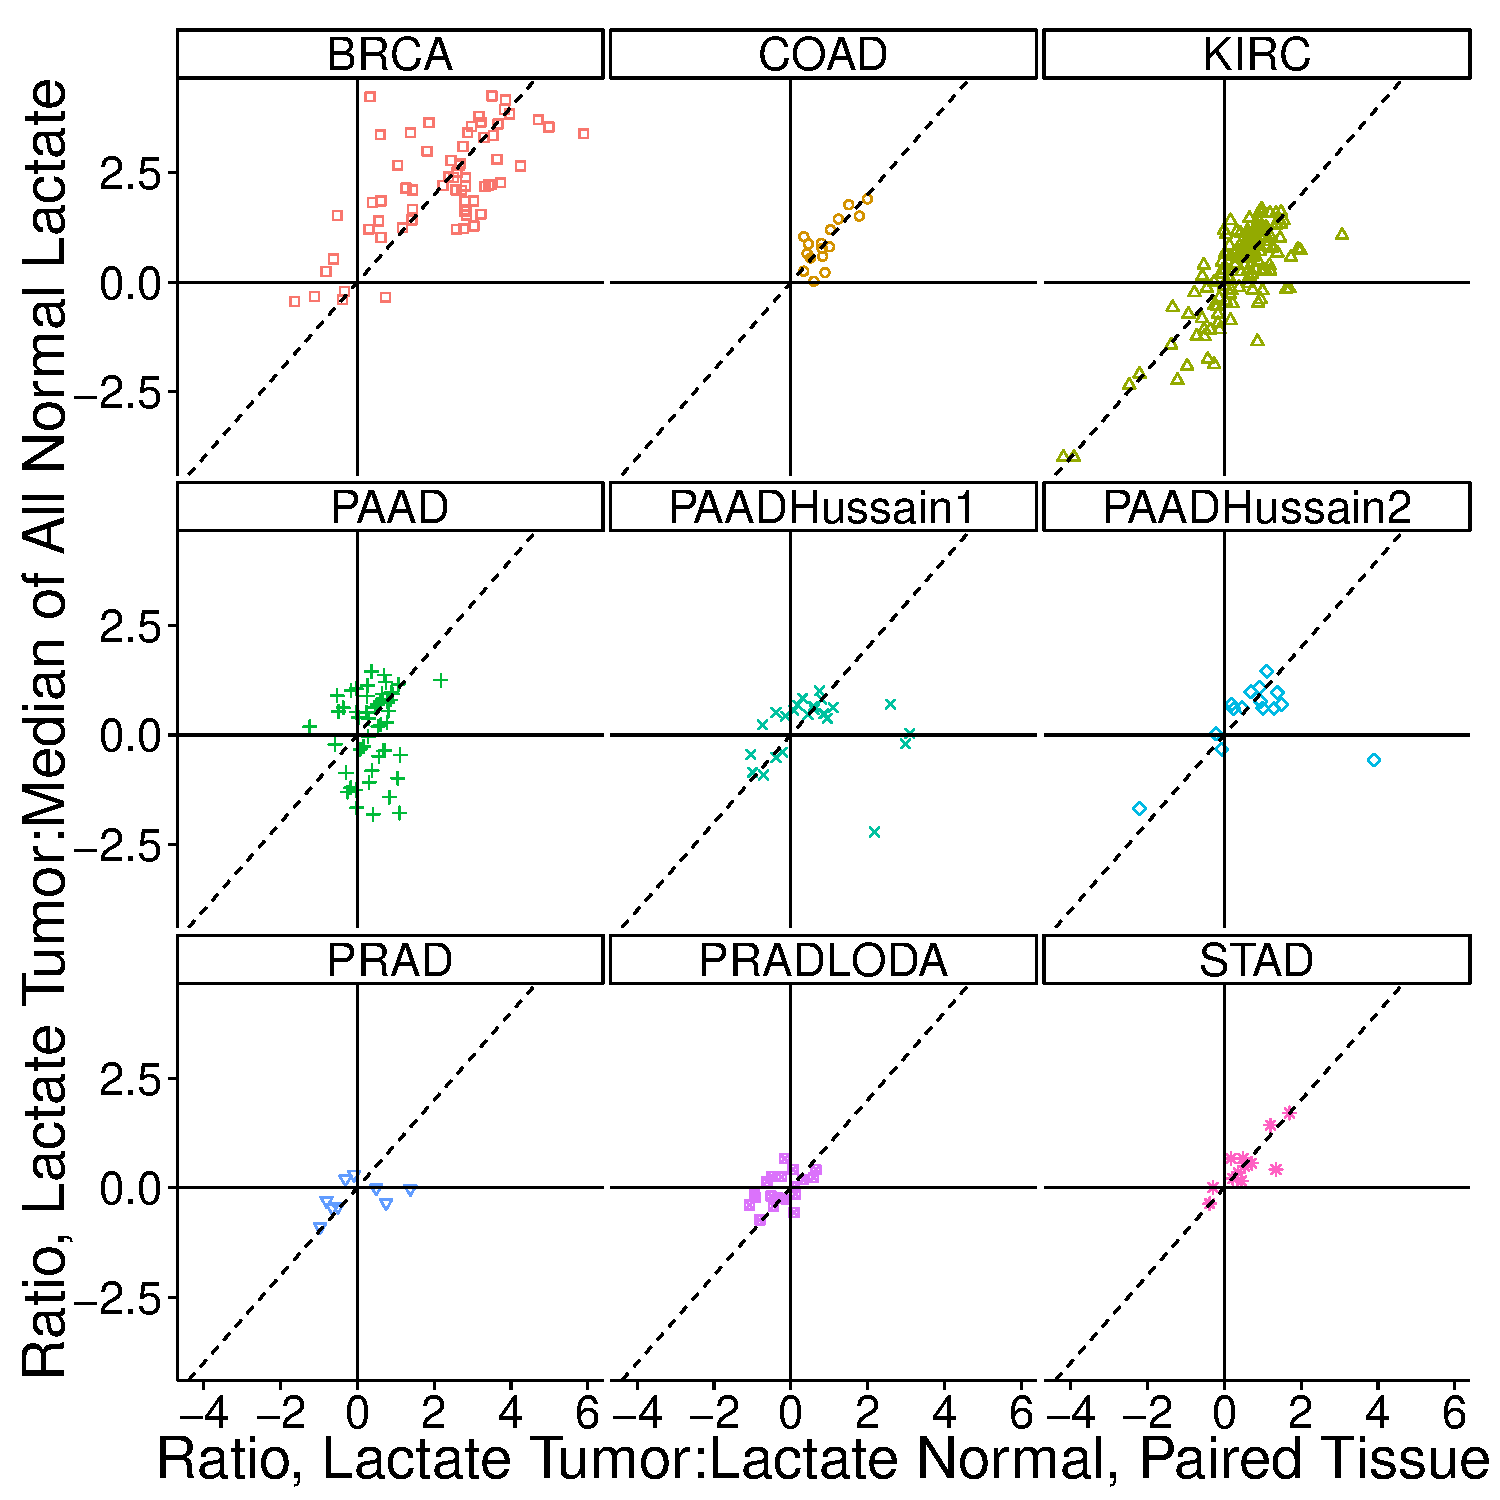
\includegraphics[scale = .6]{finalfigures/warburg_scatter.pdf}
  \caption{Insert caption.}
     \label{fig:SIFig_WarburgScatter}
\end{figure}

 
\end{document}
